\documentclass{article}
% PKGS START
\usepackage[utf8x]{inputenc}
\usepackage[english,russian]{babel}
\usepackage{cmap}
\usepackage{commath}
\usepackage{amsmath}
\usepackage{amsfonts}
\usepackage{mathtools}
\usepackage{amssymb} 
\usepackage{parskip}
\usepackage{titling}
\usepackage{color}
\usepackage{hyperref}
\usepackage{cancel}
\usepackage{enumerate}
\usepackage{graphicx}
\usepackage[a4paper, left=2.5cm, right=1.5cm, top=2.5cm, bottom=2.5cm]{geometry}
% PKGS END
% INIT START
\graphicspath{ {./images/} }
\setlength{\droptitle}{-3cm}
\hypersetup{
    colorlinks=true, %set true if you want colored links
    linktoc=all,     %set to all if you want both sections and subsections linked
    linkcolor=blue,  %choose some color if you want links to stand out
}

\pagenumbering{arabic}
% INIT END
\begin{document}
    \addtocontents{toc}{\protect\contentsline{section}{\protect\numberline{}Первый семестр}{}{}}
    \section{Понятие множества. Подмножества (включения).}

    \textbf{Обозначения.} Множества обозначают заглавными буквами латинского алфавита $(A, B, X, N)$. 
    
    Множество может задаваться двумя основными способами: 
    
    \begin{enumerate}
        \item перечислением всех элементов множества (для конечного множества); 
        \item указанием свойства, которому удовлетворяют или не удовлетворяют элементы множества (как конечные, так и бесконечные множества). 
    \end{enumerate}
    
    \textbf{Обозначения.} Элементы множества задаются строчными буквами латинского алфавита $(a, b, x)$. Принадлежность элемента множеству обозначается $a \in A$, а запись $b \not\in B$ означает, что элемент $b$ не принадлежит множеству $B$. 

    \textbf{Пример.} Рассмотрим некоторые примеры множеств. 

    $A_1 = \{0,1,2,3,4,5,6,7,8,9\}$ --— множество всех цифр;\\
    $A_2 = \{x |\ x = 2n, n \in N\}$ --— множество четных чисел;\\ 
    $A_3= \{\textrm{множество точек, равноудаленных от заданной точки}\}$;
    
    \textbf{Определение 0.} Если множество не содержит ни одного элемента, то оно называется пустым (обозн. $\emptyset$). 
    
    \textbf{Определение 1.} Говорят, что множество $B$ является подмножеством множества $A$ (обозн. $B \subset A$), если для любого $x \in B$ выполняется, что $x \in A$.\\
    Краткая запись: если $\forall\ x \in B \Rightarrow x \in A$, то $B \subset A$. 

    \textbf{Пример.}  
    
    \begin{enumerate}
        \item Если $A = \{\textrm{множество всех учеников}\}$, $B = \{\textrm{множество учеников 10-3, 10-4 классов}\}$, то $B \subset A$;
        \item Если $X = \{ x \in N |\ x\ \vdots\ 10\}, Y = \{ y \in N |\ y\ \vdots\ 5\}$, то $X \subset Y$;
        \item $\forall A, \emptyset \subset A$. 
    \end{enumerate}

    \textbf{Определение 2.} Говорят, что множества $A$ и $B$ равны $(A = B)$, если они состоят из одних и тех же элементов.\\
    $A = B \Leftrightarrow A \subset B$ и $B \subset A$.

    \textbf{Пример.}
	$A = \{(x, y): y = \abs{x-a}\}$, $B = \{(x, y): y = \sqrt{(x - a)^2}\}$, $C = \{(x, y): y = x - a\}$, $a > 0$. $A = B ?, C = B ?$\\ 
    Если $a > 0$, то $(0, a) \in B$ и $\not\in C!$

    \textit{Универсальное множество.}
    
    Бывает удобно рассматривать все множества, участвующие в каких-либо рассуждениях как подмножества некоторого фиксированного множества, которое будем называть \textit{универсальным множеством} и обозначать $E$.
    
    \textbf{Пример.}

    Если мы рассматриваем интервалы, промежутки, лучи, точки числовой прямой, то в качестве универсального множества можем рассматривать действительную ось $E = \mathbb{R}$. Тогда отрезок $[0, 1]$ можно записать как $A = \{ x \in \mathbb{R}: 0 \leq x \leq 1 \}$, а пустое множество как $\emptyset = \{x \in \mathbb{R}: x \neq x\}$.

    Свойства включений:

    \begin{enumerate}
        \item $\forall A: A \subset A$;
        \item $A \subset B,\ B \subset C \Rightarrow A \subset C$;\\
        $\uparrow$ Возьмем произвольный $x \in A$. Так как $A \subset B$, то $x \in B$. Так как $B \subset C$, то из $x \subset B \Rightarrow x \in C$. Получили, что наш $x \in C$, т.е $A \subset C. \downarrow$
        \item $\forall A: \emptyset \subset A$; 
    \end{enumerate} 

    \section{Операции над множествами. Диаграммы Эйлера-Венна.}

    Пусть даны множества $A$, $B$, $C$, универсальное множество $E$. 

    \textbf{Определение 3.} Объединением множеств $A$ и $B$ ($A \cup B$) называется множество, содержащее в себе элементы, лежащие в $A$ или в $B$. $A \cup B = \{x|\ x \in A \textrm{ или } x \in B\}$. 

    \textbf{Определение 4.} Пересечением множеств $A$ и $B$ ($A \cap B$) называется множество, содержащее в себе элементы, лежащие одновременно в $A$ и в $B$. $A \cap B = \{x|\ x \in A \textrm{ и } x \in B\}$.
    
    Если $A \cap B = \emptyset$, то говорят, что множеств $A$ и $B$ не пересекаются.  

    Удобно изображать множества и результат операций над множествами на диаграммах, которые называются диаграммами Эйлера-Венна. 

    \begin{figure}[h!]
    \centering
    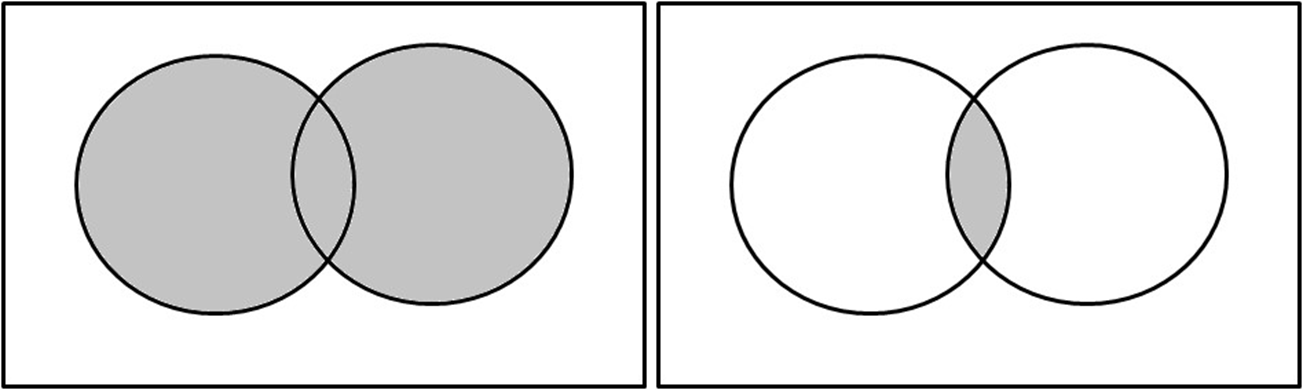
\includegraphics{1_1}
    \caption{\label{fig:fig1}Объединение (слева) и пересечение множеств (справа).}
    \end{figure}

    Свойства операций над множествами (часть 1):

    \begin{enumerate}
        \item $A \cup A = A \cap A = A$;
        \item $A \cup \emptyset = A$; $A \cap \emptyset = \emptyset$;
        \item $A \cup E = E$; $A \cap E = A$;
        \item $A \cup B = B \cup A$; $A \cap B = B \cap A$; (коммутативность или закон перестановочности)
        \item $(A \cup B) \cup C = A \cup (B \cup C)$; $(A \cap B) \cap C = A \cap (B \cap C)$; (ассоциативность или сочетательный закон)
        \item $(A \cup B) \cap C = (A \cap C) \cup (B \cap C)$; (дистрибутивность или распределительный закон)\\
        $\uparrow$ Обозначим $C_1 = (A \cup B) \cap C$, $C_2 = (A \cap C) \cup (B \cap C)$. Для доказательства равенства множеств необходимо показать два включения.\\
        Покажем, что $C_1 \subset C_2$. Пусть $x \in (A \cup B) \cap C \Rightarrow x \in A \cup B$ и $x \in C \Rightarrow x \in A$ и $x \in C$ или $x \in B$ и $x \in C$, т.е. $x \in (A \cap C) \cup (B \cap C)$.\\
        Покажем, что $C_2 \subset C_1$. Пусть $x \in (A \cap C) \cup (B \cap C) \Rightarrow x \in A$ и $x \in C$ или $x \in B$ и $x \in C \Rightarrow,\ x \in A \cup B$ (более широкое множество) и $x \in C$ или $x \in B \cup A$ (более широкое множество) и $x \in C$, т.е. $x \in (A \cup B)$ и $x \in C$ или $x \in (A \cup B) \cap C$.
        $\Rightarrow C_1 = C_2 \downarrow$
        \item Если $A \subset B$, то $A \cup B = B$, $A \cap B = A$. 
    \end{enumerate}

    \textbf{Определение 5.} Разностью двух множеств $A$ и $B$ ($A \backslash B$) называется множество, состоящее из элементов множества $A$, не принадлежащих множеству $B$. $A \backslash B = \{x|\ x \in A \textrm{ и } x \not\in B\}$. 

    \textbf{Определение 6.} Симметрической разностью множеств называется множество $A \Delta B = (A \backslash B) \cup (B \backslash A) = \{x|\ x \in A \textrm{ и } x \not\in B\} \cup \{x|\ x \not\in A \textrm{ и } x \in B\}$. 

    \begin{figure}[h!]
    \centering
    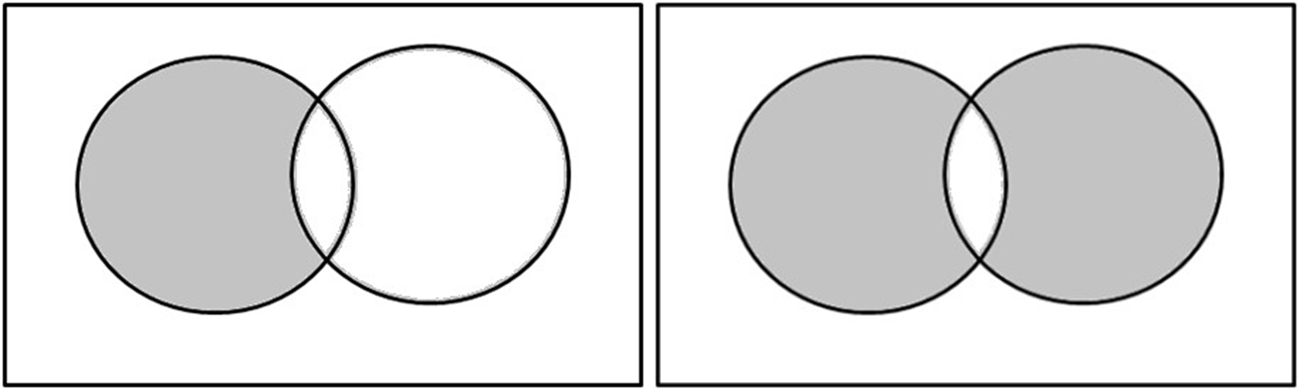
\includegraphics{1_2}
    \caption{\label{fig:fig2}Разность и симметрическая разность множеств.}
    \end{figure}

    \textbf{Определение 7.} Дополнением множества $A$ до $E$ называется множество $\overline{A} = E \backslash A$.  

    Свойства операций над множествами (часть 2):
	\begin{enumerate}
        \setcounter{enumi}{7}
        \item $A \cup \overline{A} = E$, $A \cap \overline{A} = \emptyset$;
        \item $\overline{\emptyset} = E$, $\overline{E} = \emptyset$;
        \item $(A \backslash B) \cup (B \backslash A) = (A \cup B) \backslash (A \cap B)$;\\
        $\uparrow$ Обозначим $C_1 = (A \backslash B) \cup (B \backslash A)$; $C_2 = (A \cup B) \backslash (A \cap B)$.
        \begin{enumerate}
            \item Покажем, что $C_1 \subset C_2$. Пусть $x \in (A \backslash B) \cup (B \backslash A) \Rightarrow (x \in A$ и $x \not\in B)$ или $(x \in B$ и $x \not\in A) \Rightarrow (x \in A \cup B$ (более широкое) и $x \not\in B \cap A$ (более узкое)) или $(x \in B \cup A$ и $x \not\in A \cap B) \Rightarrow x \in (A \cup B) \backslash (A \cap B)$, т.е. $x \in C_2$.
            \item Покажем, что $C_2 \subset C_1$. Пусть $x \in (A \cup B) \backslash (A \cap B) \Rightarrow x \in A \cup B$ и $x \not\in A \cap B \Rightarrow (x \in A$ или $x \in B)$ и $x \not\in A \cap B \Rightarrow (x \in A$ и $x \not\in B$ (иначе $\in A \cap B$)) или ($x \in B$ и $x \not\in A$ (иначе $\in A \cap B$)) $\Rightarrow x \in (A \backslash B)$ или $x \in (B \backslash A) \Rightarrow x \in C_1$.
        \end{enumerate}
        Из $(a),(b) \Rightarrow C_1 = C_2 \downarrow.$ 
        \item $\overline{A \cup B} = \overline{A}\cap\overline{B}$; $\overline{A \cap B} = \overline{A}\cup\overline{B}$;
    \end{enumerate}

    \section{Число элементов в объединении двух конечных множеств.}

    Обозначим $m(A)$ --— число элементов конечного множества.

    \textbf{Свойство.} $m(A \cup B) = m(A) + m(B) - m(A \cap B)$. (*) 

    $\uparrow$

    \begin{enumerate}
        \item Отметим, что $m(\emptyset) = 0$.
        \item Если $A \cap B = \emptyset$, то $m(A \cup B) = m(A) + m(B)$ (очевидно). (*) выполнена. 
        \item Пусть $A \cap B \neq \emptyset$. Рассмотрим множества $A$ и $B \backslash A$. Заметим, что $A \cup (B \backslash A) = A \cup B$ и $A \cup (B \backslash A) = \emptyset$. Тогда по свойству 2 имеем: $m(A \cup B) = m(A) + m(B \backslash A)$ (**).  
    \end{enumerate}
    
    Заметим также, что $B = (B \backslash A) \cup (A \cap B)$ и $(B \backslash A) \cap (A \cap B) = \emptyset$. Снова по свойству 2 имеем: $m(B) = m(B \backslash A) + m(A \cap B)$. Отсюда $m(B \backslash A) = m(B) - m(A \cap B)$.

    Подставляем последнее равенство в формулу (**):

    $m(A \cup B) = m(A) + m(B \backslash A) = m(A) + m(B) - m(A \cap B)$. ЧТД. $\downarrow$

    \textbf{Замечание.} Нам понадобится формула $m(A \cup B \cup C) = m(A) + m(B) + m(C) - m(A \cap B) - m(A \cap C) - m(B \cap C) + m(A \cap B \cap C)$. 

    $\uparrow$
    
    Можно доказать формулу используя доказанное свойство и свойства операций над множествами:

    $m(A \cup B \cup C) = m((A \cup B) \cup C) = m(A \cup B) + m(C) - m((A \cup B) \cap C) =$\\
    $= m(A) + m(B) - m(A \cap B) + m(C) - m((A \cap C) \cup (B \cap C)) =$\\ 
    $= m(A) + m(B) + m(C) - m(A \cap B) - [m(A \cap C) + m(B \cap C) - m(A \cap C \cap B \cap C)] =$\\
    $= m(A) + m(B) + m(C) - m(A \cap B) - m(A \cap C) - m(B \cap C) + m(A \cap B \cap C)$.
    
    Полезно рассмотреть диаграмму пересечения трёх множеств. С помощью диаграммы легко запомнить последнюю доказанную формулу:

    \begin{figure}[h!]
    \centering
    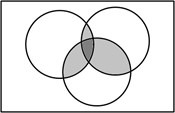
\includegraphics{1_3}
    \end{figure}

    $\downarrow$

\end{document}